\hypertarget{elektronickuxfd-derivaux10dnuxed-slovnuxedk}{%
\chapter{Elektronický derivační
slovník}\label{elektronickuxfd-derivaux10dnuxed-slovnuxedk}}

V~následující kapitole si představíme a~následně hlouběji popíšeme
výsledek praktické části, a~to nejprve v~z~hlediska požadavků na nástroj
jako takový přes jeho návrh až po samotnou implementaci.

Derivační slovník je primárně koncipován jako edukační pomůcka pro
cizince, kteří se učí češtinu jako druhý jazyk. Na rozdíl od rodilých
mluvčí nedokáží cizinci podvědomě predikovat význam neznámých slov na
základě slovotvorných morfému v~určitých kontextech -- chybí jim tedy
znalost významů určitých slovotvorných afixů, prostřednictvím kterých by
si pak dokázali analogicky vyvodit význam slova neznámého.

Díky informacím z~tohoto slovníku by tak studující mohli být schopni
odhadnout významy například takových internacionalismů, které byly
přejaty do slovotvorného systému českého jazyka pomocí sufixů. Taktéž se
očekává intuitivnější chápání derivačních pravidel u~cizinců, jejichž
rodný jazyk patří do skupiny slovanských jazyků (z~důvodu flektivního
charakteru těchto jazyků).~\parencite{adri}

\hypertarget{poux17eadavky-na-aplikaci}{%
\section{Požadavky na aplikaci}\label{poux17eadavky-na-aplikaci}}

Primárním zadáním praktické části bylo vytvořit derivační slovník ve
formě mobilní aplikace, který bude využívat slovotvorných informací
z~derivační sítě DeriNet. Dalším požadavkem, který vychází přímo z~povahy
samotného slovníku jakožto podpůrného nástroje pro výuku cizinců, bylo
vyhledat a~implementovat dvojjazyčný česko-anglický slovník, a~to proto,
aby byla celá aplikace včetně slovotvorných definic kompletně
lokalizovaná v~anglickém jazyce.

Požadavky na funkcionalitu slovníku jako takového můžeme ve stručnosti
shrnout v~následujících bodech:

\begin{itemize}
\tightlist
\item
  funkce \emph{insert word} --\textgreater{} vrátí se zadaného vstupu:

  \begin{itemize}
  \tightlist
  \item
    částečnou slovotvornou analýzu;
  \item
    anglickou i~českou definici založenou na strukturním významu slova
    (anglickou pouze v~případě, že se takový ekvivalent bude nacházet ve
    vybraném česko-anglickém slovníku);
  \item
    doplňující derivační a~morfologické informace;
  \end{itemize}
\item
  heslář již zpracovaných slov ve formě rejstříku.
\end{itemize}

Součástí zadání také bylo to, aby všechny funkcionality mobilní aplikace
byly kompletně funkční bez připojení k~internetu -- tím párem nebylo
zapotřebí řešit autentifikaci
uživatele\footnote{Nicméně je tato možnost stále v~řešení, a~to pro případ, kdybychom v~aplikaci chtěli nabídnout možnost ukládání již naučených hesel do osobního adresáře atd.}
či pracovat se vzdáleným uložištěm.

\hypertarget{nuxe1vrh-aplikace}{%
\section{Návrh aplikace}\label{nuxe1vrh-aplikace}}

Na začátku samotného vývoje si je zapotřebí určit několik věci, v~našem
případě jde primárně o:

\begin{itemize}
\tightlist
\item
  zvolení vhodných technologií včetně programovacího jazyka, kterými
  budeme nástroj implementovat;
\item
  návrh jednotlivých obrazovek aplikace a~navigaci mezi nimi (včetně
  konkrétních přechodů).
\end{itemize}

\hypertarget{pouux17eituxe9-technologie}{%
\subsection{Použité technologie}\label{pouux17eituxe9-technologie}}

Tradiční způsob vývoje mobilních aplikací se obecně dělí na tři hlavní
typy -- jde o~takzvané webové, nativní a~hybridní aplikace. Každý
z~těchto přístupů má svá vlastní pozitiva a~negativa, a~tedy si je
zapotřebí na začátku každého vývoje určit, pro jaké účely má daná
aplikace sloužit a~jaké funkcionality splňovat.

Webové aplikace fungují typicky na všech platformách a~jsou založeny na
klasických webových technologiích, tzn. na HTML, CSS a~na programovacím
jazyce JavaScript (viz podkapitola \ref{webovuxe9-technologie}), jedná
se tedy o~přizpůsobené webové stránky, z~čehož vyplývá potřeba
internetového připojení. Výhodou tohoto přístupu je kromě již zmíněné
multiplatformní povahy ukládání dat na webových serverech, tyto aplikace
tak nevyžadují velké množství paměti na lokálním uložišti. Za hlavní
negativum je považována nižší kompatibilita s~hardwarem a~operačním
systémem u~daných mobilních zařízení.

Na druhou stranu nativní aplikace jsou vyvíjeny pouze pro jednu
specifickou platformu, to znamená, že například aplikaci vytvořenou pro
systém Android nelze spustit na systému iOS a~naopak. Z~tohoto přístupu
vyplývají výhody ve formě maximálního využití daného operačního systému
(větší výkon, kompatibilita, uživatelská zkušenosti, \ldots{}), ale
i~nevýhody týkající se nutnosti využívání specifických technologií
určitého operačního systému (například pro operační systém iOS se
využívá programovací jazyk Objective-C (nově Swift), pro Android je
určen jazyk Java).

Posledním typem jsou pak hybridní aplikace, které kombinují oba předešlé
přístupy -- vývoj probíhá ve specializovaném nástroji za použití
webových technologií, v~rámci kterého se testuje logika jednotlivých
funkcionalit. Po jeho dokončení dochází ke kompilaci do vybraného
operačního systému, v~rámci kterého se již pracuje s~klasickými
nativními funkcemi (například s~mikrofonem, fotoaparátem, lokálním
uložištěm v~telefonu atd.). Výhoda hybridních aplikací je
v~jednoduchosti vývoje, který je v~porovnání s~nativním rychlý a~snadný,
a~to i~z~toho důvodu, že se u~něj pracuje pouze s~jedním zdrojem kódu,
který je použitelný na větší počet platforem. Negativním aspektem je pak
pomalejší výpočetní výkon, který je spojen s~využitím speciálních
knihoven pro převod do výsledné podoby mobilní aplikace.

Jelikož se v~našem případě pracuje s~minimem nativních funkcí, aplikace
by měla být nezávislá na internetovém připojení a~jde nám spíše
o~rozšíření nástroje napříč různými platformami, zvolíme hybridní formu
vývoje.

\hypertarget{webovuxe9-technologie}{%
\subsubsection{Webové technologie}\label{webovuxe9-technologie}}

Jak bylo výše poznamenáno, vývoj hybridních aplikací probíhá
prostřednictvím klasických webových technologií, do nichž spadá HTML,
CSS a~JavaScript, proto si je v~následujících odstavcích v~krátkosti
popíšeme.

HTML (Hypertext Markup Language) a~CSS (Cascading Style Sheets) jsou dvě
základní technologie, na nich jsou v~nejobecnější rovině postaveny
webové stránky. HTML je značkovací jazyk, pomocí kterého popisujeme
strukturu webových stránek, to znamená, že za použití speciálně
definovaných značek přiřazujeme jednotlivé významy částem obsahu. Pomocí
CSS pak nastavujeme vizuální podobu dané webové stránky (barvy, fonty,
odsazení atd.), důležitou vlastností CSS je nezávislost na HTML, tedy
můžeme dle potřeby tyto dva jazyky separovat a~následně s~mírnými
obměnami využít v~rámci jiného projektu/prostředí.~\parencite{htmlcss}

Před samotným vykreslením určité webové stránky musí dojít k~převedení
HTML dokumentu do objektu zvaného DOM (Document Object Model) -- jde
o~HTML uložené ve stromové struktuře, kde je o~každém jednotlivém uzlu
(tedy značce) uložená informace o~jeho lokaci, s~tímto objektem dále
pracuje CSS (aplikují se jednotlivá pravidla týkající se vykreslení)
a~JavaScript, prostřednictvím kterého se pak může dynamicky měnit
struktura a~zobrazení tohoto stromového objektu.
\parencite{howbrowserswork}

JavaScript (obecněji ECMAscript) je
skriptovací\footnote{Jako skriptovací jazyk je označován z~toho důvodu, že není při svém spuštění nijak kompilován (například na rozdíl od programovacích jazyků jako jsou Java nebo Objective-C) a~namísto toho je rovnou proveden daným webovým prohlížečem (ten je tak jeho interpretem).}
programovací jazyk, který je součástí všech moderních webových
prohlížečů. JavaScript se používá na takových místech, kde je zapotřebí
v~rámci webové stránky určitým způsobem interagovat s~jejím uživatelem,
to znamená, že ho typicky využijeme v~oblasti webových aplikací, u~nichž
je očekávaný zásah uživatele a~je zapotřebí dynamicky měnit zobrazovaný
obsah.~\parencite{javascript}

\hypertarget{framework-ionic-a-angular}{%
\subsubsection{Framework Ionic a~Angular}\label{framework-ionic-a-angular}}

Při vývoji komplexnějších webových a~mobilních aplikací se často pracuje
s~takzvanými webovými frameworky, které určitým způsobem zjednodušují
vývoj. Ve stručnosti je jejich účelem umožnit vývojářům práci v~takovém
prostředí, kde se můžou primárně zaměřit na požadavky daného projektu
a~nemusí řešit problematiku opakujících se funkcí nebo závislosti
jednotlivých knihoven.

My jsme v~rámci naší mobilní aplikace využili Ionic Framework, což je
soubor nástrojů s~otevřeným zdrojovým kódem pod licencí
MIT\footnote{https://opensource.org/licenses/MIT}, který se zaměřuje na
uživatelský interface u~mobilních a~webových aplikací. Obsahuje velké
množství vizuálních komponent, jež jsou typické pro mobilní zařízení,
a~taktéž je zde umožněno pomocí knihovny Ionic Native přistupovat
k~nativním funkcím mobilního zařízení -- zde se využívá knihovna Cordova,
která slouží pro převod webové aplikace do aplikace mobilní.
\parencite{cordova}

Dalším cílem Ionicu je poskytnout takové prostředí pro vývoj hybridních
aplikací, které je kompatibilní s~dalšími frameworky, jako jsou
například React nebo Vue, nicméně jeho jádro a~struktura samotného kódu
je založena na webovém frameworku Angular.~\parencite{ionic}

Angular jako takový pracuje s~programovacím jazykem TypeScript, který je
vyvíjen firmou Microsoft jako open-source. TypeScript je rozšíření již
zmíněného JavaScriptu, to v~praxi znamená, že kód napsaný v~TypeScriptu
je zapotřebí nejdříve zkompilovat (převést) do určité podoby
JavaScriptového standardu a~ten je až poté možné interpretovat ve
webových prohlížečích. Tento programovací jazyk se používá primárně
z~důvodu své silné typové kontroly, pokud je tedy této možnosti využito,
lze tak díky ní předcházet mnohým potenciálním chybám.
\parencite{typescript}

Architektura frameworku Angular se skládá z~mnoha vzájemně provázaných
vrstev, zde si ve stručnosti popíšeme právě ty, které jsou pro pochopení
naši aplikace klíčové. Základním prvkem architektury jsou
\emph{komponenty}, v~rámci kterých dochází k~propojení aplikační logiky
s~konkrétní HTML šablonou (ta určuje celkový vzhled) a~CSS. Jedna
komponenta je většinou rovna jedné vizuální stránce v~aplikaci, nicméně
Angular dokáže svými vlastními značkami (\emph{direktivami}) ovlivnit
výslednou podobou šablony ještě před jejím zobrazením -- díky tomuto
principu jednoduše dochází k~dynamické proměně obsahu stránek podle
zadané aplikační logiky, protože ta právě ovlivňuje chování samotných
direktiv. Další důležitou části jsou \emph{služby} -- ty už nejsou
propojeny s~žádnou vizuální stránkou (s~HTML šablonou), ale slouží pro
dekompozici jednotlivých funkcionalit napříč aplikací. Data, která jsou
těmito službami zpracována, jsou pak dále přeposílána do určitých
komponent.~\parencite{angulararchitecture}

\hypertarget{nuxe1vrh-obrazovek}{%
\subsection{Návrh obrazovek}\label{nuxe1vrh-obrazovek}}

\hypertarget{implementace-aplikace}{%
\section{Implementace aplikace}\label{implementace-aplikace}}

V~poslední kapitole si popíšeme architekturu předkládané aplikace spolu
s~její hlavní funkcionalitou \emph{insert word.}

\hypertarget{architektura-aplikace}{%
\subsection{Architektura aplikace}\label{architektura-aplikace}}

Mobilní aplikace se skládá z~pěti hlavních stránek (komponent), jde o:

\begin{itemize}
\tightlist
\item
  vysouvací menu;
\item
  úvodní obrazovku;
\item
  stránku s~funkcionalitou \emph{insert word};
\item
  rejstřík se zpracovanými slovy;
\item
  stránku s~informacemi o~aplikaci.
\end{itemize}

Implementačně je nejkomplexnější komponenta s~funkcionalitou
\emph{insert word}, proto se na ní v~následující části důkladněji
zaměříme a~pro demonstraci použitého algoritmu použijeme přiložené
schéma (viz obrázek \ref{algoritmus}). Pro větší přehlednost jsou na
diagramu modře zvýrazněny komponenty, žlutou barvou služby, zeleně
interní uložiště s~daty a~červeně pak hlavní funkce (ty se dále větví do
menších podfunkcí, jejichž popis není pro účely tohoto popisu klíčový).

\begin{figure}[ht]   
    \centering
    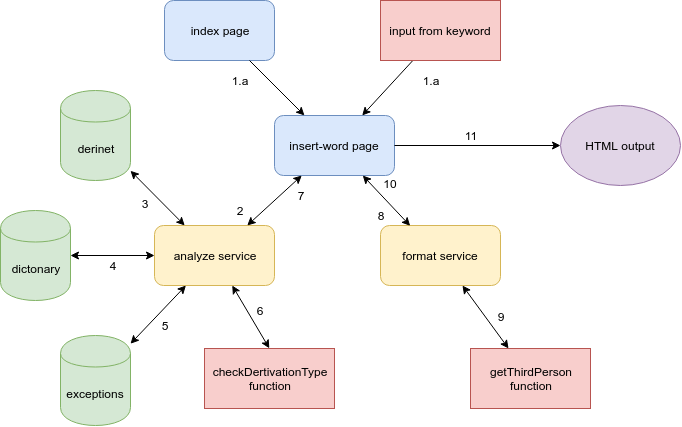
\includegraphics[width=.9\textwidth]{algoritmus}  
    \caption{Algoritmus funkcionality insert word}
    \label{algoritmus}
 \end{figure}

V~prvé řadě musí aplikace nějakým způsobem získat vstup pro následnou
analýzu, existují dva způsoby, jak k~tomu docílit -- v~případě kroku 1.a
je za vstup považováno takové slovo, které bylo vybráno v~rámci
komponenty \emph{index}, tedy je vstupní slovo vybráno na stránce
s~rejstříkem zpracovaných sufixů. Druhou možností (1.b) je zadat slovo
ručně prostřednictvím funkce \emph{fromUser} z~textového pole, v~takovém
případě se po zadání prvního písmena (a~následně dalších znaků)
vyselektují všechna slova z~rejstříku, která začínají zadaným
podřetězcem.

V~okamžiku, kdy je vybráno vstupní slovo, je tento řetězec zaslán do
služby \emph{analyze} (2), která řeší všechny záležitosti týkající se
derivační sítě DeriNet a~překladu. V~této službě se při jejím volání
inicializuje objekt, který bude cílovým výstupem této služby -- tento
objekt nazýváme \emph{infoBase} a~skládá se z~několika atributů:

\begin{itemize}
\tightlist
\item
  vstup v~českém jazyce (při inicializaci je za jeho hodnotu přiřazeno
  vstupní slovo);
\item
  vstup v~anglickém jazyce (při inicializaci je spuštěn automatický
  překlad);
\item
  slovotvorný typ (tento a~zbytek atributů zůstávají při inicializaci
  prázdné);
\item
  prefigovanost;
\item
  prefix;
\item
  derivační proces;
\item
  rod;
\item
  derivační cesta.
\end{itemize}

Při inicializaci se souběžně načítají data z~interního uložiště, která
jsou následně zkonvertována do použitelného datového formátu (3, 4, 5),
konkrétně jde o~databázi DeriNet, česko-anglický slovník
Glosbe\footnote{https://glosbe.com/ -- jedná se o~open-source projekt pod licencí CC-BY-SA z~něhož byla vyextrahována data pro naše použití.}
a~seznam výjimek (viz kapitola
\ref{zpracovanuxe9-slovotvornuxe9-sufixy}).

Dalším krokem je postupné procházení derivační sítě DeriNet, z~níž
potřebujeme vyextrahovat výše zmíněné lingvistické informace, procházíme
tedy derivační řetězec směrem od slova vstupního k~jeho slovu
základovému do té chvíle, než se zamění slovní druh, pak přistupujeme
k~volání funkce \emph{checkDertivationType} (6). Ta nám porovná řetězce
obou slov a~určí, o~jaký se jedná derivační proces a~slovotvorný typ.
Dále určuje algoritmus z~celého derivačního řetězce prefigovanost
(popřípadě zjišťuje o~jaký prefix se přesně jedná), zaznamená si rod
vstupního slova (ve výjimkách máme tedy v~případě slovotvorného sufixu
\emph{-tel} taková slova, která jsou neživotnými maskuliny) a~ukládá si
základové slovo spolu s~jeho anglickým ekvivalentem (u~českých
odvozených slov ve slovníku často překlad chybí). Posléze služba
\emph{analyze} vrací již vyplněný objekt \emph{infoBase} zpátky do
komponenty \emph{insert-word}, vrácený objekt může vypadat například
takto:

\begin{verbatim}
1.  czechInput:  "zpracovatel"
2.  czechParent:  "zpracovat"
3.  derProcess:  "suffixation"
4.  derivType:  "tel"
5.  derivationPath:  (2) [{…},  {…}] // derivační řetězec
6.  englishInput:  ""
7.  englishParent:  "processes"
8.  gender:  "M"
9.  isPrefig:  true
10. prefix:  "z"
\end{verbatim}

Nyní se dostáváme do kroku č. 8, kdy je objekt \emph{infoBase} předán
druhé službě s~názvem \emph{createDefiniton}, jejímž účelem je vytvořit
samotné slovníkové heslo do formy objektu \emph{definiton}. Jednotlivé
části jsou zpracovány separátně, a~to jednak z~důvodu přehlednosti kódu,
ale taktéž z~ryze praktické příčiny, tedy aby s~výsledným objektem byla
co nejjednodušší manipulace na úrovní HTML šablony.

Na začátku inicializujeme obecnou slovotvornou definici podle rodu ze
vstupního objektu \emph{infoBase} a~poté přistupujeme k~funkci
\emph{getThirdPerson} (9), v~rámci které vytváříme slovesnou formu ve
třetí osobě podle lingvistických pravidel popsaných v~kapitole
\ref{slovotvornuxe1-definice}.

Následně dotvoříme derivační a~morfologickou informaci z~poznatků
získaných ze služby \emph{analyze} a~vracíme objekt \emph{definiton}
zpět do komponenty \emph{insert-word} (10). Pokud je vrácen objekt
správného typu, je HTML šabloně umožněno skrze direktivy frameworku
Angular přistoupit k~jednotlivým častém definice a~vykreslit je do
označených míst v~šabloně (11).

Výhoda tohoto objektového přístupu je taková, že se na jednotlivých
jasně otypovaných místech v~kódu provádí pouze jeden specifický úkol,
a~tím je do určité míry zajištěna robustnost celkové aplikace, kdy je při
výpadku jedné služby/funkce jednoduché lokalizovat místo chyby.
